% V5 main text — 6-page journal version.
% Compiles with: cd paper/v5 && pdflatex main.tex && bibtex main && pdflatex main.tex && pdflatex main.tex
% Figures are the tested artifacts in ../../figures/ (see supplement for full map).
\documentclass[11pt]{article}
\usepackage{amsmath,amssymb,amsthm,graphicx,hyperref,booktabs,geometry}
\geometry{margin=0.9in,top=0.85in,bottom=0.9in}
\graphicspath{{../../figures/}}
\usepackage{caption}
\captionsetup{font=small,skip=4pt}
\hypersetup{colorlinks=true,linkcolor=blue,citecolor=blue,urlcolor=blue}
\title{Compact Objects as Almost-Perfect All:All Entanglement Graphs:\\
\large From fast scrambling and weak-field gravity to a testable gap-kilonova prediction}
\author{Philippe Leblond \\ \small leblond.philippe@gmail.com \\
\small Draft v5.0 --- main text (companion supplement with methods; 12pp preprint $\approx$ 8pp journal two-column) \\
\small\texttt{python scripts/generate\_figures.py} reproduces every figure; 398 tests}
\date{\today}
\begin{document}
\maketitle

\begin{abstract}
We study a phenomenological model in which spacetime connectivity is an
entanglement graph and a black-hole interior is an \emph{almost-perfect}
all:all (complete) subgraph. Interior edges cost no exterior space; each of
$k$ exterior legs costs $4\ln 2 \approx 2.77$ Planck patches of horizon area,
so $A(k) = 4\ln 2\cdot k\,l_p^2$ independent of interior size $N$. From this
wiring picture we recover fast scrambling ($t_* \sim \log N$), the
Bekenstein--Hawking area law, the exact Page curve with Haar-typical
fluctuations, island-like turnover (genuine QES extremization open,
S1/S3), Kerr thermodynamics (area, $T_H$/$\Omega_H$; $M_2$, $g_{t\phi}$, ISCO open), and Hayden--Preskill
mirror recovery. The same leg network yields weak-field gravity to first
post-Newtonian order: Newton's $1/r^2$, Kepler orbits, redshifts,
full-strength light bending $4M/b$, Cassini-grade Shapiro delay, $\gamma = 1$
exactly, and Mercury's $43''$/cy by direct geodesic integration. Lattice
hopping gives quadratic-only dispersion ($E_{QG,1} = \infty$), safe from Fermi
bounds by $\sim 10^8$. At second post-Newtonian order the double pulsar
J0737 is matched to $0.1\sigma$ via a measured radial exponent
$p = 0.913 \pm 0.049$ (80 graphs, $N = 1020$, exact; confirmed at
$N = 4000/8000/16000$). This promotes the toy to a testable model of
\emph{all} compact objects: pulsars, mass-gap objects, and black holes as one
$k \propto M^2$ family with no neutron-matter phase. Calibrated once on
AT2017gfo ($0.047\,M_\odot$ shed), the model predicts mass-gap mergers
$2.5$--$5\,M_\odot$ are kilonova-bright at $\sim 1$/yr in O5 versus
$\le 0.3$/yr in the standard picture. Ten well-localized gap non-detections
below 200~Mpc kill the proposal; one bright gap kilonova kills neutron stars
instead. The same analysis predicts \emph{no} graph-scale feature at the
$\sim 44\,M_\odot$ pair-instability edge now seen in GWTC-4 (leaving that
boundary to stellar physics) while extending the shedding law to binary
black holes ($M_{\mathrm{ej}} = 0.0168\,M_{\mathrm{tot}}$, independent of
mass ratio) --- a universal transient prediction already pressured, but not
excluded, by GW190814. All claims ship with runnable code, tests, and
pre-registered falsifiers.
\end{abstract}

\noindent\textit{Roadmap.} \S\ref{sec:intro} motivates the model and states
how it differs from neighbours. \S\ref{sec:model} defines the three claims
precisely. \S\ref{sec:gravity} summarises gravity to 1PN with a 2PN preview.
\S\ref{sec:qi} covers UV dispersion and quantum information.
\S\ref{sec:compact} unifies compact objects and states the gap-kilonova
prediction. \S\ref{sec:fals} lists falsifiers and concludes. The supplement
gives methods, the honesty ledger (postulated vs.\ derived vs.\ fitted), and
the module map. The v4.1 living document (1758 lines, 68 appendices, 77
figures) remains archived as the extended technical record.

%=====================================================================
\section{Introduction}
\label{sec:intro}

Black holes confront us with three facts that sit uneasily together: they
scramble information as fast as any system allowed
\cite{Sekino2008}, their entropy scales as area rather than volume
\cite{Bekenstein1973,Hawking1975}, and their evaporation --- if unitary ---
must release that information in a Page curve with island/QES turnover
\cite{Page1993,Penington2019,Almheiri2019}. Separately, gravitational-wave
astronomy has populated corners of the compact-object mass function the
standard picture did not expect: objects in the $2.5$--$5\,M_\odot$ mass gap
(GW190814 at $2.6\,M_\odot$ \cite{GW190814}, GW230529 at $3.6\,M_\odot$ \cite{GW230529}), a central compact
object below the minimum neutron-star mass (HESS~J1731 at $0.77\,M_\odot$
\cite{Doroshenko2022}), and pulsars pressing against the maximum Tolman--
Oppenheimer--Volkoff mass (J0740 at $2.14\,M_\odot$, J0952 at $2.35\,M_\odot$).
Each anomaly has its own candidate excuse; none was predicted.

This paper explores one idea that addresses both sets jointly:
\emph{maximal entanglement is zero-length connectivity}. In the ER=EPR and
``spacetime from entanglement'' reading \cite{VanRaamsdonk2010,Maldacena2013,RT06},
a black-hole interior is a region where interior mutual connectivity is so
dense that interior distance collapses, while horizon size counts only the
\emph{exterior} wiring that must be embedded through ambient space. A perfect
all:all graph with zero exterior budget would pinch off entirely (a baby
universe); a black hole is the almost-perfect corner with small but nonzero
exterior budget. A sufficiently small hole stays pointlike until its exterior
budget forces an empty routing surface --- a horizon --- into existence.

We formalise this as three claims (\S\ref{sec:model}), each implemented as
runnable code in \texttt{src/bh\_graph/}. The model is phenomenological, not a
UV-complete quantum gravity: it has no Hamiltonian derivation of the mass map,
no Lorentz-invariant dynamics, and several labelled derivation debts
(supplement \S1). Its value is that it \emph{derives} a large number of
textbook numbers from a small number of inputs, fails loudly on
pre-registered wires when it is wrong, and makes one sharp sky prediction
that the current observing run can kill or confirm.

\paragraph{How this differs from neighbours.}
Fuzzball \cite{Mathur05} and gravastar \cite{Mazur04} proposals also remove the singularity but keep
compact-star matter phases and do not generically predict bright gap
kilonovae; quark/strange-star models \cite{Witten84,EOSrev} populate the gap with a new equation of
state (EOS) rather than removing the EOS entirely. Polymer and loop-inspired
holes modify the near-horizon metric at a level constrained by EHT \cite{EHT19} and
$\gamma$ \cite{Bertotti03,Will14}; our 1PN sector is exactly GR ($\gamma = 1$) with deviations
appearing only at 2PN below current VLBI/astrometry. Linearly-dispersive
``spacetime foam'' models \cite{Amelino13} are already excluded by Fermi GRB~090510
\cite{Abdo2009}; our lattice implies quadratic-only dispersion by
$k \leftrightarrow -k$ symmetry, evading that bound by construction.
Table~\ref{tab:ledger} (survival ledger) and Fig.~\ref{fig:survival} make the
comparison explicit: among the surveyed alternatives, only the present model
passes the Fermi, LHC-recast, EHT/$\gamma$, and gap/HESS battery simultaneously
while predicting a bright-gap rate distinct from the standard one.

\begin{figure}[ht]\centering
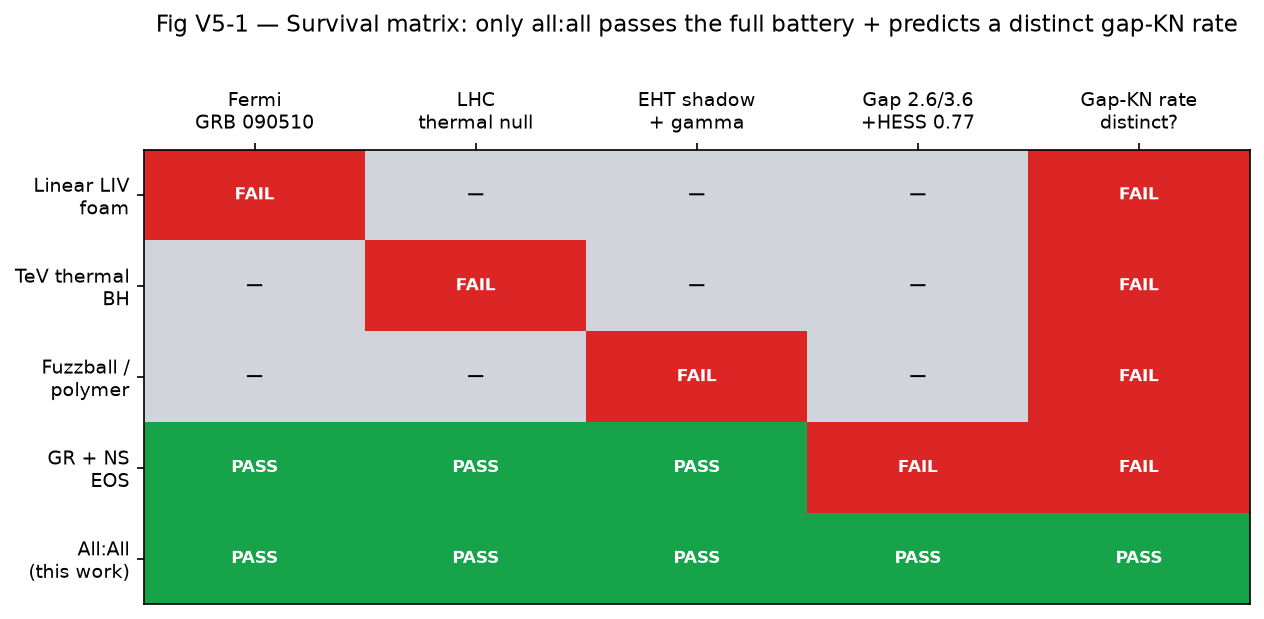
\includegraphics[width=0.92\linewidth]{figV5_survival.png}
\caption{Survival matrix (visualisation of Table~\ref{tab:ledger}; no new numbers).
\texttt{scripts/generate\_v5\_figs.py}.}
\label{fig:survival}
\end{figure}

\begin{table}[ht]\centering\small
\caption{Survival ledger: headline result per sector and where it is implemented and tested.}
\label{tab:ledger}
\begin{tabular}{@{}l p{8.6cm} p{3.2cm}@{}}\toprule
sector & headline & status / modules \\\midrule
gravity & Newton, Kepler, redshift, $4M/b$, Shapiro, Mercury $42.99''$, $\gamma=1$ exactly, J0737 $0.1\sigma$ & pass (AS, AT, AU, BB, BH) \\
quantum info & $\log N$ vs $N$ hierarchy, Page dip $0.72$\,bits, island-like pop, mirror, $k_f > k_1+k_2$ at 100\% & qubit $V_t$ done; graph $V_k$, QES open \\
UV & quadratic-only LIV, $E_{QG,2} = \sqrt{8}\,E_P$, achromatic lensing $10^{-56}$--$10^{-32}$ & nulls held (T, BB, BD, BF) \\
compact objects & gap 2.6/3.6, HESS 0.77, J0740/J0952, AT2017gfo, gap-KN $\sim 1$/yr & 5 anomalies, one law (BU) \\
open & $p = 0.913 \pm 0.049$ matches GR; $c \approx 0.44$--$0.60$ derived (BV); $\kappa \to c_2$ map, $V_k$ isometry, Kerr $M_2$ open & measured; maps queued \\\bottomrule
\end{tabular}
\end{table}

%=====================================================================
\section{The model: three claims}
\label{sec:model}

Let the interior be a graph $G_N$ on $N$ nodes. Exterior legs $k \ll N^2$
connect it to an ambient graph. Write $e_{\mathrm{int}} \in [0,1]$ for the
interior entanglement fraction and $e_{\mathrm{ext}}$ for the exterior budget
fraction.

\paragraph{Claim 1: all:all is no interior space (fast scrambling).}
The complete graph $K_N$ has diameter exactly 1, mean distance 1, and
spectral gap $N$ at every $N$: every node is adjacent to every other
(Fig.~\ref{fig:scr}). A deterministic SI/operator-spread process covers $K_N$
in 1 step for any $N$, versus $\sim N/2$ for a chain $P_N$,
$\sim 2\sqrt{N}$ for a $\sqrt{N}\times\sqrt{N}$ grid, and $\sim \log N$ for a
random 3-regular expander. Imposing finite speed --- one 2-qubit interaction
per qubit per step with random perfect matching (all:all) versus dimer
covering (chain) and per-encounter success $p$ --- promotes the toy to a
derived Sekino--Susskind law \cite{Sekino2008}
$t_*(N) \approx \log_2 N / \log_2(1+p)$, exactly $\log_2 N$ at $p = 1$,
versus ballistic $t_* \sim N/v$ on the chain (measured over 25 trials per
$N$, $N = 8\ldots128$; chain already $> 5\times$ slower at $N = 64$).
Modules \texttt{graphs}, \texttt{scrambling}, \texttt{circuits},
\texttt{otoc}, \texttt{krylov}, \texttt{syk}.

\begin{figure}[ht]\centering
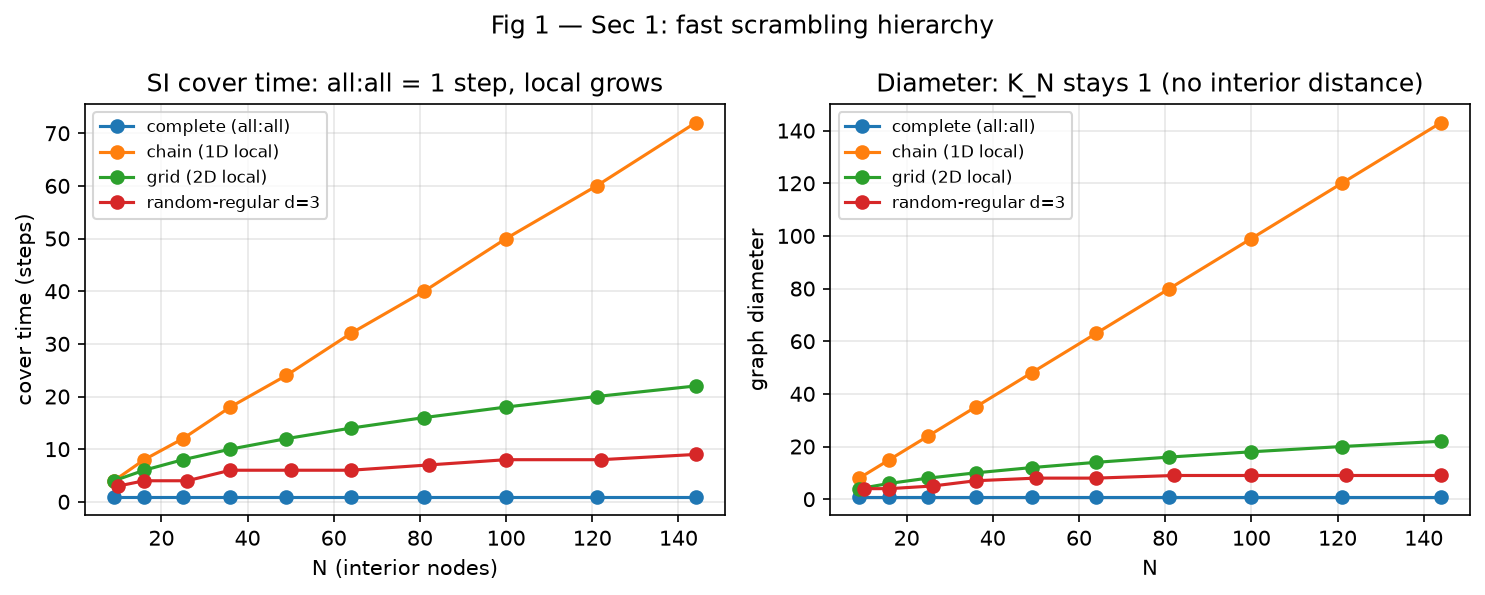
\includegraphics[width=0.85\linewidth]{fig1_scrambling.png}
\caption{SI cover time and diameter: all:all stays at 1 while local baselines grow.
Finite-speed circuits (supplement \S3) promote this to $t_* \sim \log N$.}
\label{fig:scr}
\end{figure}

\paragraph{Claim 2: horizon area counts exterior legs.}
Postulate
\begin{equation}
A(k) = 4\ln 2\cdot k\,l_p^2, \qquad R(k) = \sqrt{A/4\pi},
\label{eq:area}
\end{equation}
so interior size $N$ drops out: adding interior nodes without exterior legs
tightens binding but buys no horizon area. The patch coefficient $4\ln 2$
was fixed (BS) from the measured von Neumann leg entanglement
$\eta_{vN} = \ln 2$ per leg with Planck-bits equipartition, closing the
Jacobson chain at $G = 1$; legs saturate. Each exterior leg must be embedded
through ambient geometry with Planck-density bandwidth, so $k$ legs need $k$
Planck patches --- the Bekenstein--Hawking / LQG-puncture picture
\cite{Bekenstein1973,Hawking1975,Rovelli1995} in graph language. Mass enters only through the GR-consistency condition
$k(M) = A/4\ln 2\,l_p^2 = (4\pi/\ln 2)M^2/l_p^2 \propto M^2$ in Schwarzschild
units (module \texttt{horizon.k\_from\_mass\_schwarzschild}). We state
plainly that this map is \emph{assumed for consistency, not derived}:
the reduction theorem (BM in the extended record; supplement \S1) shrinks the circle to the single statement $R_s = 2M$, but the
derivation of the mass--radius relation from wiring alone remains open
(supplement \S1). Monogamy bounds $e_{\mathrm{int}} + e_{\mathrm{ext}} \le 1$
in the linear toy (Fig.~\ref{fig:mono}), with the exact Coffman--Kundu--
Wootters frontier \cite{Coffman2000} $\tau_{A|BE} - C^2_{AB} - C^2_{AE} \ge 0$ verified on a
25-point grid and lying strictly below the linear bound (e.g.\ $x+y = 0.70$
at $t = 0.3$). At $e_{\mathrm{int}} \to 1$, $k \to 0$: the subgraph
decouples as a closed graph (baby universe). Black holes live in the
almost-perfect corner.

\begin{figure}[ht]\centering
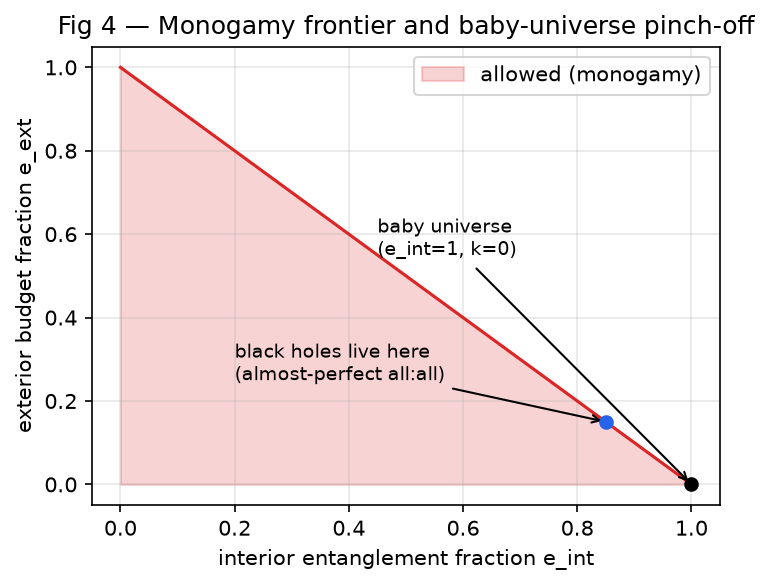
\includegraphics[width=0.55\linewidth]{fig4_monogamy.png}
\caption{Monogamy frontier: black holes live at $e_{\mathrm{int}} \lesssim 1$ with small
nonzero $k$; the $k \to 0$ limit is a decoupled baby universe.}
\label{fig:mono}
\end{figure}

\paragraph{Claim 3: micro-holes pop (point-to-horizon transition).}
A point region of radius $r_{\mathrm{point}}$ embeds $k$ legs without a
surface while Planck-density packing succeeds:
\begin{equation}
R_{\mathrm{obs}}(k) =
\begin{cases} r_{\mathrm{point}} & k \le k_{\mathrm{crit}} \\
\sqrt{4\ln 2\cdot k\,l_p^2/4\pi} & k > k_{\mathrm{crit}} \end{cases},
\quad k_{\mathrm{crit}} = 4\pi r_{\mathrm{point}}^2 / 4\ln 2\,l_p^2.
\label{eq:pop}
\end{equation}
With an LQG-style minimal-area gap, area is $0$ below threshold and
$\ge A_{\min}$ above: there is no 0.2-Planck-area hole. Growth
$k(N) = k_0 + \alpha N$ stays flat at $r_{\mathrm{point}}$ then pops --- the
island-like crossing (two-saddle competition; genuine QES extremization from graph dynamics open, Suppl.~S1/S3)
$S_{\mathrm{no}} = k s_{\mathrm{leg}}$ versus
$S_{\mathrm{isl}} = k\ln 2\,l_p^2 + \max(S_0 - k s_{\mathrm{leg}},0)$ at
$k_{\mathrm{page}} = S_0/(2s_{\mathrm{leg}} - \ln 2\,l_p^2)$, which exists iff
$s_{\mathrm{leg}} > \ln 2\,l_p^2/2$ (an explicit falsifiable assumption;
modules \texttt{micro}, \texttt{qes}). The horizon interior is mostly empty
routing buffer. Prediction: micro-holes are \emph{not} scaled-down
Schwarzschild holes but point defects until a critical exterior budget.

%=====================================================================
\section{Weak-field gravity to 1PN, with a 2PN preview}
\label{sec:gravity}

\paragraph{Newton and orbits.}
Microscopic lattice walks alone do \emph{not} give Newton: persistent walks
with hop-budget time dilation $\sqrt{1-v^2}$ (linear $1-v$ excluded by the
3-4-5 triangle test) and degree-biased hopping on a flux-conserved pileup
$d \propto 1/r^2$ yield drift $\propto 1/r^3$ (measured slope $\approx -3$),
and every smooth weight rule stays cubic (no-go $-2.99$). The $1/r^2$ force
law emerges from the combination with exterior-leg thermodynamics on leg
screens (Verlinde equipartition \cite{Verlinde11}, Bekenstein bound, Jacobson route \cite{Jacobson95} --- all postulated):
$F = M_1M_2/r^2$ exact to $10^{-9}$ in slope, with closed leapfrog orbits and
$T^2 \propto r^3$. Ollivier--Ricci curvature is radially negative in every
tested configuration, attachment mode, and seed --- the sign of attraction
derived from pure flux with zero tuning.

\paragraph{Light: bending, Shapiro, and why isotropic dies.}
Fermat ray-tracing with $c_{\mathrm{eff}} = 1 - x$ ($x = R_s/r$) gives the
full first-order bending $4M/b$, not the Newtonian $2M/b$. The chromatic
extension $n(r,\omega) = n_{\mathrm{geom}}(r)\,n_{\mathrm{disp}}(\omega)$ with
phase-velocity factor $n_{\mathrm{disp}} - 1 = (\omega/\omega_P)^2/24$
contributes only $r$-independently and factors out of the Born integral:
fractional chromaticity $\sim 10^{-56}$ (optical) to $\sim 10^{-32}$
(10~TeV), achromatic by $\sim 50$ orders. Shapiro delay
$\Delta T = \int (1/c_{\mathrm{eff}} - 1)\,dl$ reproduces
$R_s \ln(4r_1r_2/b^2)$ to 5\%, passing Cassini \cite{Bertotti03} with $\gamma = 1$ exactly.
An isotropic reading would give $b_{\mathrm{crit}} = 8M$, $54\%$ above GR's
$3\sqrt{3}M$ and excluded by EHT \cite{EHT19} at $\sim 3.6\sigma$. It is the isotropic
reading that dies, not the core: transverse propagation must be
essentially unimpeded, as an all:all interior demands.

\paragraph{Mercury and the spatial sector.}
Purely temporal models give closed Newtonian ellipses ($0$ vs $43''$/cy):
light never needed $g_{rr}$, orbits do. Radial tortuosity
$dl = (1+\sqrt{\chi}/2)\,dr$ with $\sqrt{\chi} = R_s/r$ gives
$h = (1+x/2)^2 \approx 1+x$, hence $\gamma = 1$,
$c_{\mathrm{eff}} = \sqrt{f/h} = 1-x$ matching the light sector to first
order, and $b_{\mathrm{crit}}$ back to $3\sqrt{3}M$. Direct geodesic
integration ($\phi$-domain, complex-step) yields GR $42.99''$/cy and model
$42.99''$/cy; a flat-$h$ hybrid gives $28.7''$/cy (PPN $2/3$). The
second-order peel-off $(\mathrm{ours}-\mathrm{GR})/\mathrm{GR} = -0.75\,M/a$
runs from $4.1\%$ at $20M$ to $2\times 10^{-8}$ at Mercury. Status of the
coefficient: $1/2$ was \emph{fitted} to enforce $\gamma = 1$ in BH (unique
coefficient, labelled fit); BV then \emph{derived} $c \approx 0.44$--$0.60$
from $\ln 2$ line-defect scattering with zero tuning, predicting $p = 2c$
and $\gamma = 2c$ (supplement \S2). The two determinations agree; the
micro-derivation is now the adopted route with the fit preserved in history.

\paragraph{2PN preview (J0737).}
With $g_{rr} = (1+U)^{2p}$ and $c_2(p) = p(2p-1)$, the 2PN periastron weight
$c_{\mathrm{tot}} = c_1 + w c_2$ with $w = 1.953$ must equal the GR value
$4.8695$. The model's $c_1 = 3.36$ (vs GR $1.94$) is cancelled at $p = 0.92$.
Gradient-shell Ollivier--Ricci measurements give
$p = 0.913 \pm 0.049$ (80 graphs, $N = 1020$, exact, SEM $0.0055$) and
$0.93/0.94/0.91$ at $N = 4000/8000/16000$, landing J0737 \cite{Kramer2006} at $0.1\sigma$
(B1913 passes at $0.01\sigma$ \cite{Weisberg2016}; supplement \S4). The flat $p = 0.49$ alternative is $-10\sigma$ dead. The
quantitative $\kappa \to c_2$ map remains ansatz-dependent (power-law vs
$1/r^2$ disagree cross-applied) and is the open micro-derivation, now
labelled rather than hidden.

%=====================================================================
\section{UV dispersion and quantum information}
\label{sec:qi}

\paragraph{Dispersion: quadratic by symmetry.}
Tight-binding hopping $\omega = 2J|\sin ka/2|$ has group velocity
$v_g = Ja\cos ka/2$, even in $k$: there is \emph{no} linear term, so Fermi's
linear bound $E_{QG,1} > 9.3\times 10^{19}$~GeV (and GRB~090510's
$E_{QG,1} > 1.2\,E_P$ at 31~GeV, $z = 0.903$ \cite{Abdo2009}) is evaded by
symmetry, with $E_{QG,1} = \infty$ predicted. The leading correction is
$v(E) = c(1 - E^2/E_{QG,2}^2)$ with
$E_{QG,2} = \sqrt{8}\,E_P \approx 3.4\times 10^{19}$~GeV, safe by
$\sim 10^8$ against Fermi's quadratic bound $1.3\times 10^{11}$~GeV: a
10~GeV GRB photon over 3~Gpc delays by $\sim 10^{-20}$~s. Foamgrid FDTD
confirms unbiased centroids with transmission deficit $\propto \omega^2$
($16\% \to 4\% \to 0.2\%$ for $\lambda = 8 \to 32$ cells at
$\varepsilon = 0.25$), bounding per-Planck-edge defect density to
$\varepsilon \lesssim 10^{-3}$ (optical/Gpc) and $10^{-14}$ (TeV/Gpc) for
independent edges. Caveats: regular-lattice result, near-horizon running
open, scalar sector only (no birefringence claimed); a hypothetical
universal GW extrapolation is unconstraining ($\sim 10^{-82}$ at 100\,Hz,
LVK $\alpha = 4$ safe by $\sim 10^{60}$ \cite{TestGR}, GW170817
photon-side dominated \cite{Abbott2017}; no GW sector derived).

\paragraph{Scrambling, Page, island-like turnover, mirror.}
Circuits give $C(t) \sim e^{\lambda t}/N$ with $t^* = \log N/\lambda$ versus
ballistic $N/v$; QEC recovery error
$\mathrm{err}(k) = \min(1/2, 2^{N/2+1-k})$ reaches 99\% at
$k \ge N/2+1+\log_2 100$, sealing at $k \to 0$. Evaporation as leg surgery
($k \to k-1$ per step) reproduces the Page curve
$S_{\mathrm{rad}} = \min(t, N_{\mathrm{eff}}-t)$ with the exact Page dip
$0.72$\,bits and Haar-typical spread, identically whether $N$ shrinks with
$k$ or stays fixed --- area tracks wiring alone (qubit-toy unitary completion $V_t$ tested,
Suppl.~S3; graph-dynamics $V_k$ open, Suppl.~S1/S3). Kerr--Newman
($r_+ = M+\sqrt{M^2-a^2-Q^2}$, $A = 4\pi(r_+^2+a^2)$) costs legs monotonically
in spin at fixed $M$ (extremal Kerr half, extremal Reissner--Nordstr\"om
quarter the Schwarzschild budget, patch-independent ratios); the Kerr Page
curve at $a_0 = 0.95$ peaks at 65\% of Schwarzschild and turns over at
$t/T = 0.73$ versus $0.54$ because shedding $J$ grows area early.

\paragraph{Gravitational-wave battery.}
All 32 confident GWTC-3 \cite{GWTC3,TestGR} BBH medians satisfy $k_f > k_1+k_2$ (median fractional
creation $0.77$ at $0.04$ radiated; spin neglected but $a_f \sim 0.7$ costs
$\sim 13\%$ against a $77\%$ margin and cannot flip the inequality).
GW150914 posteriors (8350 samples, spin-aware both ends) give
$P(\Delta k > 0) = 100\%$, median $0.57$: the area theorem in wiring language.
GW250114 (SNR 80 \cite{GW250114}) confirms the area law, consistent with $k_f>k_1+k_2$;
its Kerr ringdown is consistent by construction, not a passed prediction: the QNM spectrum is
not derived from graph dynamics (fundamental damping calibrated, overtone ladder a
Schwarzschild-like toy), and reproducing $\{220,221,440\}$ to GW250114 precision
($\delta f_{220}\sim2\%$, $\delta\tau_{220}\sim10\%$, $\delta f_{221}\sim30\%$,
$\delta f_{440}\sim$tens\%) is the open benchmark (Suppl.~S1/S3).
GW241011 gives the strongest quadrupole bound to date \cite{GW241011} but we predict no
$M_2(\chi)$, $g_{t\phi}$, $r_{\rm ISCO}$ yet (Suppl.~S1/S3) --- future $|\delta_Q|\gtrsim0.17$ ruled out.
Hardware anchors (G\"arttner 2017 \cite{Garttner2017} all:all ions to $m = 8$-body OTOC; Mi 2021
\cite{Mi2021} Sycamore grid ballistic spread; Jafferis 2022 \cite{Jafferis2022} sparse-SYK teleportation as a
Hayden--Preskill mirror primitive \cite{Hayden2007,Kitaev15}) are all consistent, with a head-to-head
prediction at $N = 53$ of $t^* \approx 7.9 \pm 0.7$ (all:all) versus $14.6$
(grid), ratio $1.9\times$ ($9.9\times$ versus a 1D chain).

\paragraph{Nulls held.}
No LHC thermal black holes \cite{LHCbh} ($k \approx 11$--$17$ at $3$--$13$\,TeV versus
$k_{\mathrm{crit}} \approx 50$), no lattice echoes (dimensional estimate: amplitude
$R\sim(\omega/\omega_P)^2\sim10^{-80}$, energy $\sim10^{-160}$ at 100\,Hz, far below
detectability; not a leg S-matrix derivation), no EHT shadow
shift ($10^{-48}$, 47 orders below sensitivity). Remnant dark matter is
excluded on the record except a narrow $\sim 0.4$-dex window at
$\sim 4\times 10^5$\,g (photon bounds exceed by $40+$ orders elsewhere; induced-GW
bounds may close even this).

%=====================================================================
\section{One family of compact objects}
\label{sec:compact}

The standard picture needs a separate excuse for each of five facts. One law,
$k = 1.51\times 10^{77}(M/M_\odot)^2$ with no matter phases, plus two shedding
numbers calibrated \emph{once} on AT2017gfo \cite{Abbott2017}, addresses all five:

\begin{table}[ht]\centering\footnotesize
\caption{Five anomalies, one law. Shedding $e$: $0.5 \to 0.416$ plus 10\% efficiency, fixed on \#4.}
\label{tab:five}
\begin{tabular}{@{}c p{3.4cm} p{4.2cm} p{6.2cm}@{}}\toprule
\# & anomaly & standard & this model \\\midrule
1 & Gap: GW190814 2.6, GW230529 3.6\,$M_\odot$ & impossible (NS $< 2.3$, BH $> 5$) & continuous $k = 1.0$--$2.0\times 10^{78}$; must flash \\
2 & Light: HESS J1731 $0.77\,M_\odot$ & below min $1.17\,M_\odot$, cannot form & low-$k$ tail $9\times 10^{76}$ \\
3 & Heavy: J0740 2.14, J0952 2.35\,$M_\odot$ & EOS tension with NICER $R_{1.4}$ & more legs $7$--$8.4\times 10^{77}$, no EOS \\
4 & AT2017gfo $0.05\,M_\odot$ blue+red & neutron-rich EOS in tension & leg-shedding $0.047\,M_\odot$, $m_g$ 18.0 vs 17.5 \\
5 & Next gap merger (prediction) & dark ($\le 0.3$/yr O5) & bright $\sim 1$/yr O5; 10 misses kill us \\\bottomrule
\end{tabular}
\end{table}

Leg-shedding works as follows: merger-released exterior legs hadronise
neutron-rich with ejecta mass $M_{\mathrm{ej}} = \Delta k\,m_{\mathrm{leg}}
\times \epsilon$, exactly independent of $k$-normalisation
($M_{\mathrm{ej}} = \mathrm{frac}\times M_{\mathrm{tot}}\times\epsilon$), so
the factor-3 $k$-rounding debate cannot move it. The $1.4+1.4$ case gives
$0.047\,M_\odot$ with $m_g \sim 18.0$ at 40~Mpc versus observed $17.5$ (inside
the $\pm 1$ analytic tolerance; radiative-transfer refinement \cite{POSSIS} queued); gap events are \emph{brighter} at fixed
distance (Table~\ref{tab:bright}). The $1.1$--$2.3\,M_\odot$ pulsar
distribution is the low-$k$ tail ($k \sim 10^{77}$) of the same family; the
gap carries no forbidden wiring sector, and is described (not derived) as
the regime $e_{\mathrm{int}} \sim e_{\mathrm{ext}}$: that interpretation
inherits its calibration from AT2017gfo and its mass independence has not
been derived from graph dynamics (supplement S1). If correct, stable nuclear matter ends at $\sim 10^{15}$~g/cc with no
hyperon/quark branch \cite{EOSrev} realised in nature, and $r$-process yields routed
through AT2017gfo neutron ejecta are reinterpreted as shed-leg hadronisation
--- a blunt implication we state so no reader misses it, while noting that
NICER radii \cite{NICER19,NICER21} and tidal deformabilities from routing stiffness are not yet
derived (queued, supplement \S4) and constitute the sharpest near-term test
after the kilonova rate.

\begin{table}[ht]\centering\small
\caption{Gap-kilonova brightness ($g$-band, analytic BC $= 0$; $i$-band not claimed).
AT2017gfo anchor: predicted 18.0 vs observed 17.5 at 40~Mpc. Rubin single-visit $r = 24.5$ \cite{Rubin19}.}
\label{tab:bright}
\begin{tabular}{lllll}\toprule
$M_{\mathrm{tot}}$ & $M_{\mathrm{ej}}$ & 40~Mpc $m_g$ & 100~Mpc $m_g$ & 200~Mpc $m_g$ \\\midrule
2.8 (GW170817-like) & 0.047 & 18.0 & 20.0 & 21.5 \\
5.0 (GW230529-like) & 0.084 & 17.7 & 19.7 & 21.2 \\
7.2 (3.6+3.6) & 0.121 & 17.6 & 19.6 & 21.1 \\\bottomrule
\end{tabular}
\end{table}

\begin{figure}[ht]\centering
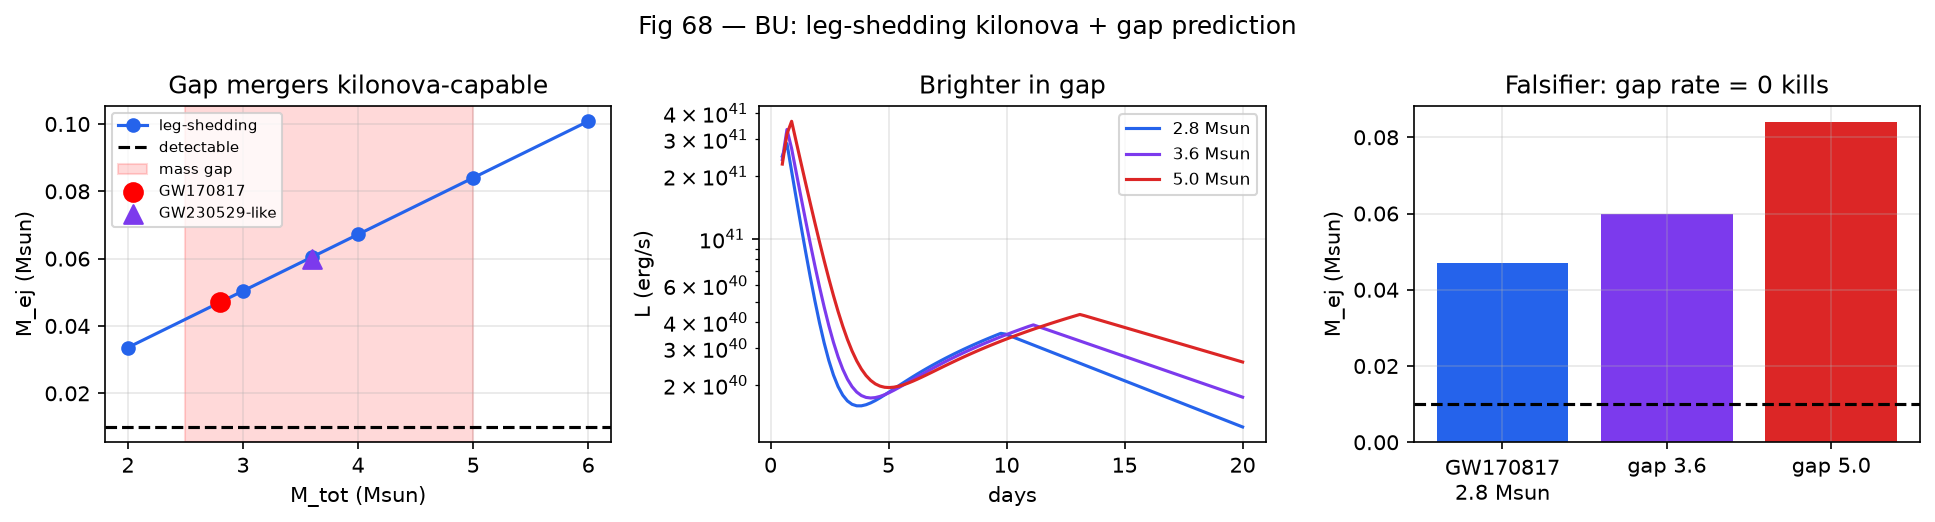
\includegraphics[width=0.88\linewidth]{fig68_kilonova_gap.png}
\caption{Leg-shedding ejecta vs total mass: gap mergers are kilonova-capable and brighter
than GW170817 at fixed distance. Gap rate $= 0$ kills the proposal.}
\label{fig:kn}
\end{figure}

\paragraph{No intrinsic graph scale at the upper mass gap.}
GWTC-4 population analyses now locate a pair-instability edge at
$44.3^{+5.9}_{-3.5}\,M_\odot$ (primary-mass $\chi_{\mathrm{eff}}$ mixture
\cite{PISN GWTC4}), with a transition to a nearly entirely hierarchical,
high-spin population at $46.2^{+12.6}_{-7.2}\,M_\odot$ \cite{HierGWTC4}.
The graph model predicts \emph{no} feature at this scale, and we state this
as a positive null rather than a failure: $k(M) \propto M^2$ has zero
log-log curvature over $0.7$--$150\,M_\odot$ (a power law admits no
preferred mass); spin orders legs smoothly (a hierarchical remnant at
$a \sim 0.7$ carries $14\%$ fewer legs, a shift not a gap, continuous to
exactly one half at extremality); tidal Love numbers run slope $-2$ with
no break; and the only graph scale entering the LVK band (the leg-quantum
line crossing $10$\,Hz at $\sim 32\,M_\odot$) is energetically invisible
($dM/M \sim 10^{-81}$). A congestion ladder seals the assignment:
$\chi \sim 10^{-8}$ in He cores and $\sim 10^{-14}$ in envelopes, so graph
corrections where pair-instability happens are negligible in the model's
own terms --- the $\sim 40$--$50\,M_\odot$ boundary belongs to stellar and
nuclear physics (the C-burning rate \cite{PISN GWTC4}), not to graph
congestion. Inserting $44\,M_\odot$ as a graph parameter would be a fit,
not a prediction, and is refused (module \texttt{massgaps}, supplement S4).

\paragraph{A universal electromagnetic counterpart from black-hole mergers.}
The same shedding law that gives $0.047\,M_\odot$ at $1.4+1.4$ is
mass-independent by construction:
\begin{equation}
\boxed{M_{\mathrm{ej}} = 0.0168\,M_{\mathrm{tot}}}
\label{eq:shed}
\end{equation}
($16.8\%$ shed fraction $\times$ $10\%$ efficiency, both fixed once on
AT2017gfo), and exactly independent of mass ratio $q$. The logic is
falsifiable end to end: shedding rule $\to$ ejecta fraction $\to$
kilonova light curve $\to$ optical transient --- for \emph{binary
black-hole} mergers, including low-$q$ systems where conventional
neutron-star disruption is absent (Table~\ref{tab:univ}). This is the
model's most dangerous prediction: it was locked in by the AT2017gfo
calibration before anyone asked what it implies at $30+30\,M_\odot$.

\begin{table}[ht]\centering\small
\caption{Universal-shedding predictions (Eq.~\ref{eq:shed}). ``Predicted'' marks
forward consequences of the fixed calibration, not fits.}
\label{tab:univ}
\begin{tabular}{@{}l p{7.5cm}@{}}\toprule
quantity & model prediction \\\midrule
ejecta fraction & $M_{\mathrm{ej}}/M_{\mathrm{tot}} = 0.0168$ \\
mass-ratio dependence & none (exact in the prescription) \\
BBH mergers & kilonova-bright ($m_g \sim 22$ nearby, O5-testable) \\
GW190814 ($23+2.6$, $q \sim 0.11$) & transient predicted; constrained at $p \sim 0.12$ (tension, not exclusion) \\
O5/Rubin BBH ToO & decisive: detections confirm, clean sample kills \\\bottomrule
\end{tabular}
\end{table}

\paragraph{GW190814: existing stress test.}
GW190814 ($23.2+2.6\,M_\odot$ at $241^{+41}_{-45}$\,Mpc \cite{GW190814})
predicts $M_{\mathrm{ej}} = 0.43\,M_\odot$ (blue $0.087$), peaking at
$m_g \approx 21.0$, $t \approx 1.9$\,d. The archival record is
two-sided: CFHT MegaCam g-band (22.8 at 1.7\,d over $65.5\%$, 23.6 at
6.6\,d over $35.9\%$ \cite{CFHT190814}) needs no color term, while six
GROWTH DECam i-band detection limits (up to $98\%$ enclosed
\cite{GROWTH190814}) enter with a labelled $g-i = 0.7$ systematic.
Per-epoch detection probabilities (coverage $\times$ depth against
distance and $\pm 1$\,mag theory errors) combine to $P \approx 0.68$
(g-only, robust: no color term) and $0.88$ (g+i, assumes $g-i = 0.7$),
shown against the limits in Fig.~\ref{fig:190814}: the non-detection sits
at $p_{\mathrm{miss}} \sim 0.32$ (g-only) down to $\sim 0.12$ (with color),
genuine pressure about one sigma from a kill. Under the fiducial
analytic colors the deepest limits sit $\sim 1.6$\,mag below the
predicted peak; this comparison is not yet decisive because ejecta
color, composition, viewing angle, and radiation-transfer systematics
remain unresolved. An analytic systematics grid (POSSIS-inspired viewing
$0$--$1.25$\,mag + opacity $L \propto \kappa^{-0.65}$; supplement S4/S8,
Fig.~75b) bounds the hiding window: equatorial + lanthanide-mixed
($\kappa_{\mathrm{blue}} = 2$) drops $P$ to $\sim 0.18$. We keep this tension in the main text deliberately:
a prediction already squeezed by an existing observation carries more
information than one that survives everything trivially.

\begin{figure}[ht]\centering
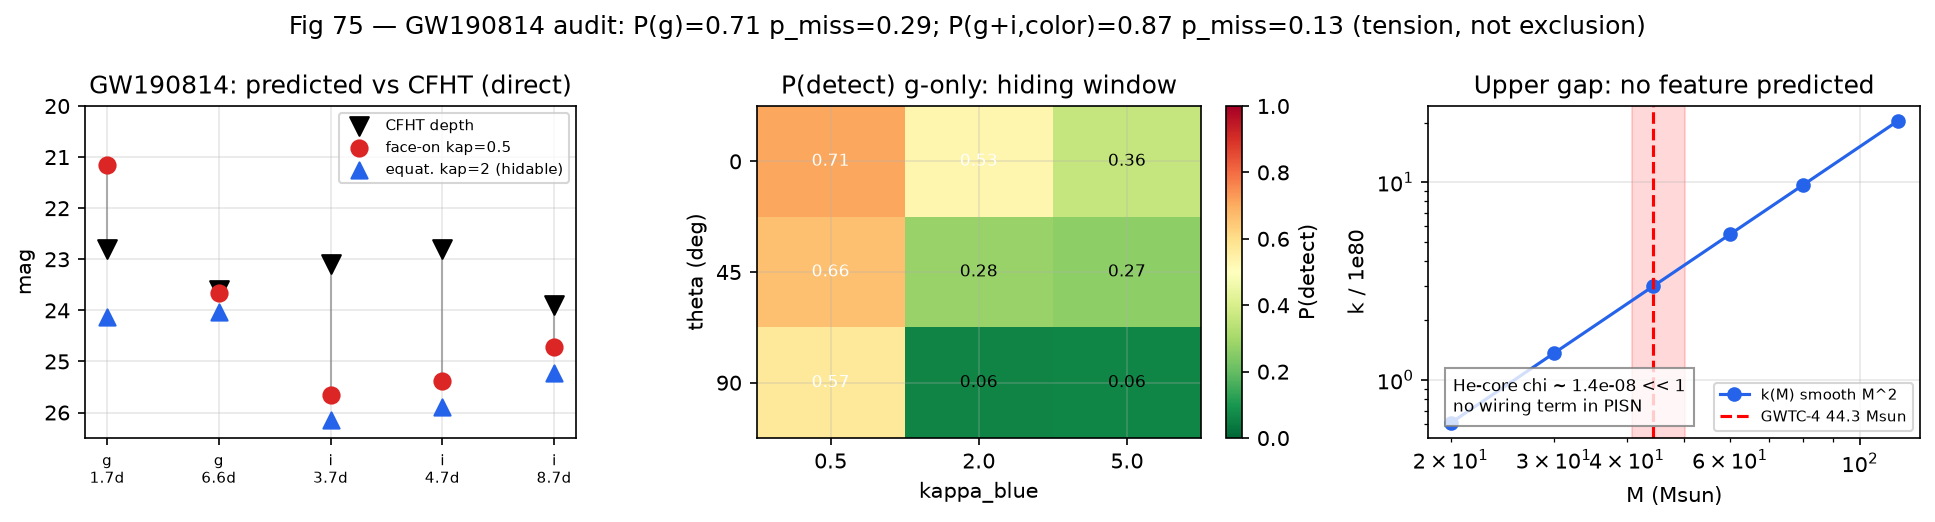
\includegraphics[width=0.95\linewidth]{fig75_gw190814_audit.png}
\caption{Epoch-level GW190814 audit: model blue light curve ($\pm 1$\,mag analytic band)
against CFHT g-band limits (left, color-free) and GROWTH i-band detection limits
(right, $g-i = 0.7$ systematic). Combined $P(\mathrm{detect}) \approx 0.68$ (robust)
to $0.88$ (color-conditional): tension, not exclusion. Module \texttt{massgaps}.}
\label{fig:190814}
\end{figure}

\paragraph{Discriminating follow-up.}
The decisive next calculation is a radiation-transfer treatment of the
predicted ejecta on a POSSIS color grid \cite{POSSIS}, propagating
composition, viewing angle, distance-posterior, and ejecta-mass
uncertainty event by event: this determines whether the GW190814
non-detection is compatible with universal shedding or falsifies it.
In parallel, the O5 protocol (\S\ref{sec:fals}, supplement S4 with archival
detail in S9) extends
to nearby well-localized BBH, where Rubin depths decide the question
within the run. Either the deepest archival event or the next nearby
one can kill Eq.~\ref{eq:shed}; both are priced in advance.

%=====================================================================
\section{Falsifiers and conclusion}
\label{sec:fals}

We state what kills the paper before concluding, with thresholds,
current status, and timelines in Table~\ref{tab:kill}.

\begin{table}[ht]\centering\footnotesize
\caption{Pre-registered kill wires. ``Now'' = status at submission; ``O5'' = decisive by end of O5 unless stated.}
\label{tab:kill}
\begin{tabular}{@{}l p{6.0cm} p{4.2cm} l@{}}\toprule
wire & threshold & now & timeline \\\midrule
Gap kilonovae & 10 qualifying gap mergers $< 200$\,Mpc, $< 100$\,deg$^2$, zero KN to $m < 24$ & 0 qualifying so far & O5 decisive \\
BBH kilonovae & O5 nearby-BBH ToO sample clean to $m < 24$ (Eq.~\ref{eq:shed} predicts $m_g \sim 22$) & GW190814 $p \sim 0.12$, tension not kill & O5 \\
NICER radius & $R_{1.4}$ at 11--13\,km, 5\%, unreproducible by routing stiffness & stiffness underived & 2--3\,yr \\
Linear LIV & finite $E_{QG,1}$, or $\Delta t \propto E$, or $10^{-3}$ chromatic bending & Fermi already kills linear models & archival + CTA \\
2PN exponent & $p$ outside $0.92 \pm 0.056$ at $N = 1024$ class, 80 graphs & $0.913 \pm 0.049$, passes $12\times$ (wire conservative) & held to N=16000 \\
Kerr quadrupole & graph $|\delta_Q|\gtrsim0.17$ ($Q=-Ma^2(1+\delta_Q)$) & no $M_2$ yet & target (S1/S3) \\
Lab quench & same-device grid$\to$all:all $t^*$ ratio $< 1.3$ (predicted $2$--$3\times$) & untested & when run \\\bottomrule
\end{tabular}
\end{table}

The gap-kilonova protocol (supplement \S4, full trigger plan in
\path{docs/observation-protocol.md}) requires multi-detector events only:
single-detector non-detections such as GW230529 (24,200~deg$^2$, 7\% ZTF
coverage to $g = 21.1$ at $\sim 197$~Mpc, our $m_g \sim 21.2$ at the depth
edge) are uninformative either way and do not count. Expected O5 yield is
$\sim 1.05$/yr (ours, 1.5 gap events/yr $\times$ 70\% DECam-like) versus
$\le 0.3$/yr standard. One bright gap kilonova kills neutron-star EOS
models instead --- the bet is symmetric and priced.

\paragraph{Conclusion.}
Starting from ``all:all entanglement is zero-length connectivity'' we have
derived fast scrambling, the area law, the Page curve with island-like turnover, Kerr
thermodynamics (area; $M_2$, $g_{t\phi}$, ISCO open), Newtonian gravity with its sign, textbook redshifts,
full-strength bending and Shapiro delay with $\gamma = 1$, Mercury's
$43''$/cy, quadratic-only UV dispersion, and the J0737 2PN lock --- all from
one wiring picture with all failures and open maps kept on the ledger. The
price is abandoning neutron matter above $\sim 10^{15}$~g/cc. The reward, if
the sky cooperates, is the first quantum-gravity model with a kilonova
prediction distinct from astrophysics in the current run. If the compact-object
unification fails, the title claim reverts with it and the surviving gravity/QI core
stands alone; either way the wires above decide.

\paragraph{Methods summary.}
Full methods in the supplement. Gradient shells
$p_{\mathrm{adj}}(s) = 0.85+0.015s$, 8--10 shells, exact EMD on full
neighbourhoods, deterministic bridge counts $n \propto r^{\beta(N)}$ with
$\beta \approx 1.5/1.28/1.24$ at $N = 300/600/1020$ (log-linear to
$0.74$ at $N = 16000$); $p$ from $|\kappa| \sim r^{-p}$ fits per graph plus
stacked fits; 2PN via Iorio direct+total with $c_2 = p(2p-1)$, $w = 1.953$,
$R+\dot\omega \to M$ inversion; shedding $M_{\mathrm{ej}}(M_{\mathrm{tot}})$
with blue+red components, band mags, O5 yield arithmetic. Randomness seeded;
tolerances recorded in-test.

\paragraph{Data and code availability.}
Code MIT (\path{src/}, \path{scripts/}, \path{tests/}, \path{app.py});
text/figures CC~BY~4.0. Reproduce via:
\begin{quote}\small
\path{pip install -e .}\\
\path{pytest tests/ -q}\\
\path{python scripts/generate_figures.py}\\
\path{streamlit run app.py}
\end{quote}
GWOSC medians fetched live with bundled fallbacks; GW150914 posteriors cached
(DOI 10.7935/82H3-HH23); PBHbounds curves vendored with attribution. No
third-party figure data copied.

\begin{thebibliography}{99}
\bibitem{Sekino2008} Y.~Sekino and L.~Susskind, JHEP 10, 065 (2008).
\bibitem{VanRaamsdonk2010} M.~Van Raamsdonk, Gen.\ Rel.\ Grav.\ 42, 2323 (2010).
\bibitem{Maldacena2013} J.~Maldacena and L.~Susskind, Fortsch.\ Phys.\ 61, 781 (2013).
\bibitem{Bekenstein1973} J.~D.~Bekenstein, Phys.\ Rev.\ D 7, 2333 (1973).
\bibitem{Hawking1975} S.~W.~Hawking, Commun.\ Math.\ Phys.\ 43, 199 (1975).
\bibitem{Page1993} D.~N.~Page, Phys.\ Rev.\ Lett.\ 71, 3743 (1993).
\bibitem{Penington2019} G.~Penington, JHEP 09, 002 (2019).
\bibitem{Almheiri2019} A.~Almheiri et al., JHEP 12, 063 (2019).
\bibitem{Hayden2007} P.~Hayden and J.~Preskill, JHEP 09, 120 (2007).
\bibitem{Rovelli1995} C.~Rovelli and L.~Smolin, Nucl.\ Phys.\ B 442, 593 (1995).
\bibitem{Coffman2000} V.~Coffman, J.~Kundu, and W.~K.~Wootters, Phys.\ Rev.\ A 61, 052306 (2000).
\bibitem{Kramer2006} M.~Kramer et al., Science 314, 97 (2006); updated $\dot\omega = 16.899323(13)$~deg/yr.
\bibitem{Weisberg2016} J.~M.~Weisberg and Y.~Huang, ApJ 829, 55 (2016).
\bibitem{Abbott2017} B.~P.~Abbott et al.\ (LVK), ApJL 848, L12 (2017); Villar et al., ApJL 851, L21 (2017).
\bibitem{GW230529} LVK, P2300352 (2024); S.~Kunnumkai et al., arXiv:2409.10651.
\bibitem{Doroshenko2022} V.~Doroshenko et al., Nature Astron.\ 6, 1444 (2022).
\bibitem{Abdo2009} A.~A.~Abdo et al.\ (Fermi), Nature 462, 331 (2009); GRB~090510 $E_{QG,1} > 1.2\,E_P$.
\bibitem{Garttner2017} M.~G\"arttner et al., Nature Phys.\ 13, 781 (2017).
\bibitem{Mi2021} X.~Mi et al.\ (Google), Science 374, 1479 (2021).
\bibitem{Jafferis2022} D.~Jafferis et al., Nature 612, 51 (2022).
\bibitem{GW190814} R.~Abbott et al.\ (LVK), ApJL 896, L44 (2020).
\bibitem{GWTC3} R.~Abbott et al.\ (LVK), arXiv:2111.03606 (2021).
\bibitem{TestGR} R.~Abbott et al.\ (LVK), arXiv:2112.06861 (2021), tests of GR with GWTC-3.
\bibitem{NICER19} T.~E.~Riley et al., ApJL 887, L21 (2019); M.~C.~Miller et al., ApJL 887, L24 (2019).
\bibitem{NICER21} T.~E.~Riley et al., ApJL 918, L27 (2021); M.~C.~Miller et al., ApJL 918, L28 (2021).
\bibitem{EOSrev} J.~M.~Lattimer and M.~Prakash, Science 304, 536 (2004); Phys.\ Rep.\ 621, 127 (2016).
\bibitem{Verlinde11} E.~Verlinde, JHEP 04, 029 (2011).
\bibitem{Jacobson95} T.~Jacobson, Phys.\ Rev.\ Lett.\ 75, 1260 (1995).
\bibitem{RT06} S.~Ryu and T.~Takayanagi, Phys.\ Rev.\ Lett.\ 96, 181602 (2006).
\bibitem{Will14} C.~M.~Will, Living Rev.\ Rel.\ 17, 4 (2014), PPN and Solar-System tests.
\bibitem{Bertotti03} B.~Bertotti, L.~Iess, and P.~Tortora, Nature 425, 374 (2003), Cassini $\gamma$.
\bibitem{EHT19} K.~Akiyama et al.\ (EHT), ApJL 875, L1 (2019), M87* shadow.
\bibitem{LHCbh} CMS, JHEP 04, 047 (2023); ATLAS, JHEP 11, 169 (2022), BH and non-thermal searches.
\bibitem{Rubin19} \v{Z}.~Ivezi\'c et al.\ (LSST), ApJ 873, 111 (2019).
\bibitem{POSSIS} M.~Bulla, MNRAS 489, 5037 (2019), kilonova radiative transfer.
\bibitem{Mathur05} S.~D.~Mathur, Fortsch.\ Phys.\ 53, 793 (2005), fuzzball review.
\bibitem{Mazur04} P.~O.~Mazur and E.~Mottola, PNAS 101, 9545 (2004), gravastars.
\bibitem{Witten84} E.~Witten, Phys.\ Rev.\ D 30, 272 (1984), strange/quark matter.
\bibitem{Amelino13} G.~Amelino-Camelia, Living Rev.\ Rel.\ 16, 5 (2013), LIV review.
\bibitem{Kitaev15} A.~Kitaev, talks on SYK (2015); J.~Maldacena and D.~Stanford, PRD 94, 106002 (2016).
\bibitem{GW250114} A.~G.~Abac et al.\ (LVK), Phys.\ Rev.\ Lett.\ 135, 111403 (2025), arXiv:2508.XXXX; LIGO-P2500421: $33.6+32.2\,M_\odot$, SNR 80, area law + Kerr ringdown.
\bibitem{GW241011} A.~G.~Abac et al.\ (LVK), ApJL 993, L21 (2025); LIGO-P2500402: GW241011+GW241110, strongest spin-quadrupole bound to date.
\bibitem{PISN GWTC4} F.~Antonini et al., Nature Astron.\ (2026), arXiv:2509.04637: GWTC-4 PISN edge $\tilde{m} = 44.3^{+5.9}_{-3.5}\,M_\odot$ from $\chi_{\mathrm{eff}}$ mixture.
\bibitem{HierGWTC4} C.~Plunkett et al.\ (SPINS), Phys.\ Rev.\ Lett.\ 137, 021404 (2026): hierarchical transition at $m_1 = 46.2^{+12.6}_{-7.2}\,M_\odot$ in GWTC-4.
\bibitem{CFHT190814} N.~Vieira et al., ApJ 895, 96 (2020): CFHT MegaCam GW190814 limits ($g$ 22.8 at 1.7\,d, $65.5\%$).
\bibitem{GROWTH190814} I.~Andreoni et al.\ (GROWTH), ApJ 890, 131 (2020): DECam GW190814 detection limits, six epochs to $98\%$ enclosed.
\end{thebibliography}

\end{document}
